\section{Calculus III}

\subsection{Optimization}

We often want to know where our functions are at their maximum or minimum. We do this in two steps. First, wherever the first derivative is at 0, means we are either at a minimum or maximum. Second, depending upon the direction of the second derivative, we can tell if we are at a maximum or minimum. 

\begin{figure}[ht]
    \centering
    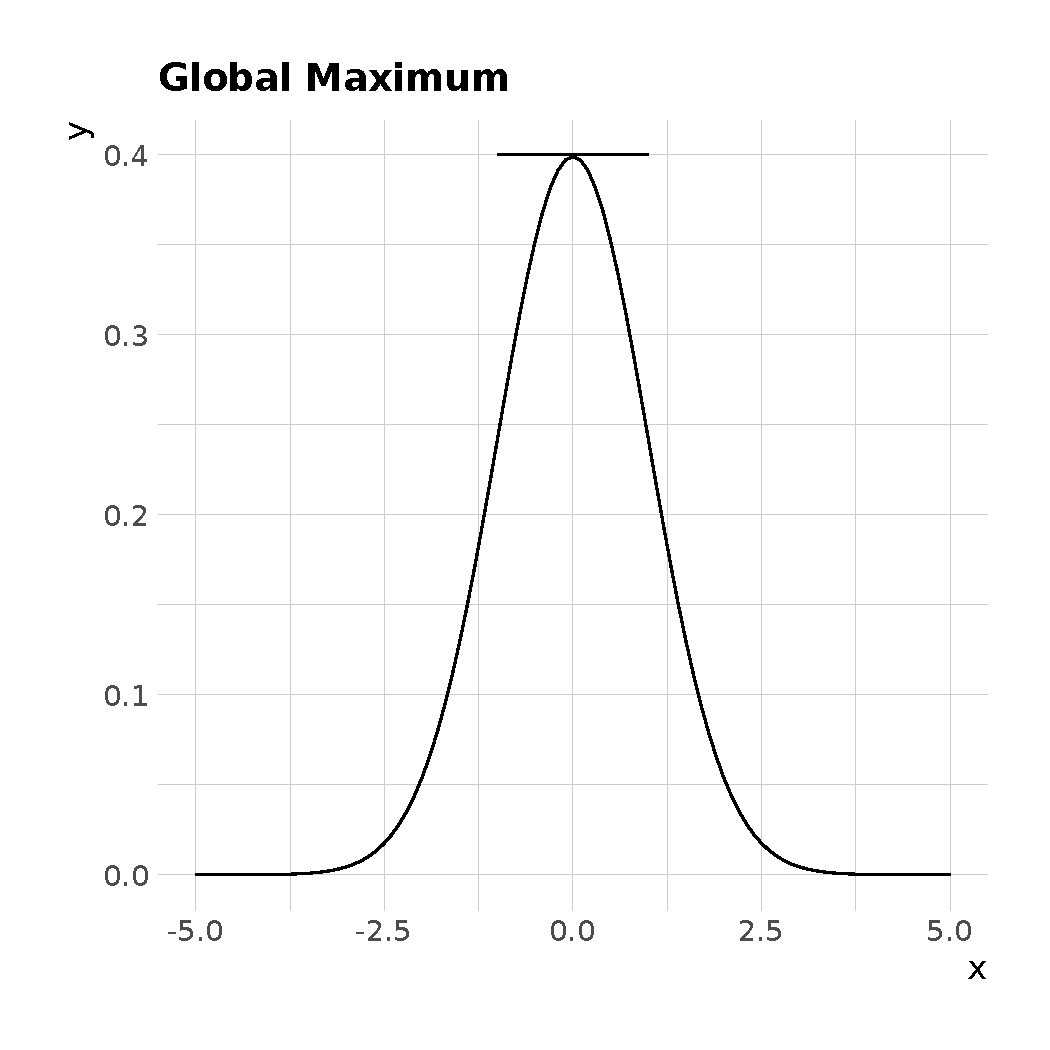
\includegraphics[scale = 0.55]{figures/optim.pdf}
    \caption{Visualizing how a derivative is equal to 0 at a function's maximum or minimum.}
    \label{fig:optim}
\end{figure}

\begin{itemize}
    \item \textbf{First-order condition}: $f'(x) = 0$
    \begin{itemize}
        \item Maximum or minimum
        \item This assumes that $f(x)$ is differentiable at all values -- it is a continuous function.
    \end{itemize}
    \item \textbf{Second-order condition}: $f''(x)$, where $>0$ means minimum, $<0$ means maximum, and $=0$ an inflection point.
\end{itemize}

\begin{align*}
    f(x) & = x^2 - 4x -1 \\
    \text{FOC: } f'(x) & = 2x -4 \\
    x & = 2 \\
    \text{SOC: } f''(x) & = 2 \Rightarrow \text{minimum}
\end{align*}

\noindent What if we have multiple variables?

\begin{itemize}
    \item Let $f(x) = -x_1^2 + x_1x_2 - x_2^2$ 
    \begin{itemize}
        \item FOC: 
        \begin{itemize}
            \item $f_{x_1} = -2x_1 + x_2 = 0$
            \item $f_{x_2} = x_1 - 2x_2 = 0$ 
            
            \vspace{1em}
            $\begin{bmatrix}[cc|c]
                    -2 & 1 & 0 \\
                    1 & -2 & 0
            \end{bmatrix}$
            \vspace{1em}

            \begin{itemize}
                \item It turns out $x_1 = 0$, $x_2 = 0$
            \end{itemize} 
        \end{itemize} 
        \item SOC: We need to build the hessian:
        
        \vspace{1em}
        $\begin{bmatrix}
            \frac{d^2f}{dx_1x_1} & \frac{d^2}{dx_1x_2} \\ \\
            \frac{d^2f}{dx_2x_1} & \frac{d^2f}{dx_2x_2}
        \end{bmatrix}
        = 
        \begin{bmatrix}
            -2 & 1 \\
            1 & -2
        \end{bmatrix}
        $
        \vspace{1em}
    \end{itemize}
    \item Now, we ask whether these points are minima, maxima, indeterminate, or saddle points. 
    \begin{itemize}
        \item We calculate the determinants of each ``principal minor''.
        \item PM$_1 = -2$, $D_1 = -2$
        \item PM$_2 = \begin{bmatrix}
            -2 & 1 \\
            1 & -2
        \end{bmatrix}$, $D_2 = (-2 \cdot -2) - (1 \cdot 1) = 3$
    \end{itemize}
    \item The hessian is:
    \begin{itemize}
        \item Positive definite: $D_1 > 0$, $D_2 > 0$, strictly local minima
        \item Negative definite: $D_1 < 0$, $D_2 > 0$, strictly local maxima
        \begin{itemize}
            \item Start negative and then alternate signs
        \end{itemize} 
        \item Positive semi-definite: $D_1 \geq 0$, $D_2 \geq 0$
        \item Negative semi-definite: $D_1 \leq 0$, $D_2 \geq 0$
    \end{itemize}
    \item For larger matrices?
    \begin{itemize}
        \item $\begin{bmatrix}
            .
        \end{bmatrix}$, PM$_1 = $ determinant of $1 \times 1$
        \item $\begin{bmatrix}
            . & . \\
            . & .
        \end{bmatrix}$, PM$_2 = $ determinant of $2 \times 2$
        \item $\begin{bmatrix}
            . & . & .\\
            . & . & . \\
            . & . & .
        \end{bmatrix}$, PM$_3 = $ determinant of $3 \times 3$
    \end{itemize}
    \item If we have a $3 \times 3$ matrix:
    \begin{itemize}
        \item PD: D$_1 > 0$, D$_2 > 0$, D$_3 > 0$
        \item ND: D$_1 < 0$, D$_2 > 0$, D$_3 < 0$
        \item PSD: D$_1 \geq 0$, D$_2 \geq 0$, D$_3 \geq 0$
        \item NSD: D$_1 \leq 0$, D$_2 \geq 0$, D$_3 \leq 0$
    \end{itemize}
\end{itemize}


\subsection{Constrained Optimization -- Lagrange Multiplier}

Sometimes, we have to find the maxima or minima under set conditions. 

\begin{align*}
    & \text{Max } f(x_1, x_2) \text{ s.t. } g(x_1, x_2) = 0 \\
    & \text{Max } f(x_1, x_2) - \lambda g(x_1, x_2)
\end{align*}

\begin{itemize}
    \item $\lambda$ is us creating a new variable.
    \item FOC: 
    \begin{align*}
        f_{x_1} - \lambda g_{x_1} = & \, 0 \\
        f_{x_2} - \lambda g_{x_1} = & \, 0 \\
        g(x_1, x_2) = & \, 0 \\
    \end{align*}
        \item Then:
    \begin{align*}
        f(x_1, x_2) = & 36 - x_1^2 - x_2^2, \, \, g(x_1, x_2) = x_1 + 7x_2 - 25  \\ 
        f(x_1, x_2, \lambda) = & 36 - x_1^2 - x_2^2 - \lambda(x1 + 7x_2 - 25) \\
        f_{x_1} & = -2x_1 - \lambda = 0, \Rightarrow x_1 = -\lambda/2 \\
        f_{x_2} & = - 2x^2 - 7\lambda = 0, \Rightarrow x_2 = -7\lambda/2 \\
        g(x_1, x_2) & = -\lambda/2 + -7\lambda/2 - 25 = 0 \\ 
        \lambda & = -1 \\
        \text{Therefore: } & x_1 = \frac{1}{2}, x_2 = \frac{7}{2} 
    \end{align*}
\end{itemize}

\subsection{Integration}

\begin{itemize}
    \item $f(x) = 40x$
    \item $F(x) = 20x^2 + c$
    \begin{itemize}
        \item This is the `antiderivative', $F'(x) = f(x)$, because if $F(X)$ is derived then it returns $f(x)$.
        \item We add c because any constant will turn to 0 when the derivative is taken. 
    \end{itemize}
    \item Powerfully, antidifferentiation lets us solve for the value of $y$, given $dy/dx$.
\end{itemize}

\begin{itemize}
    \item \textbf{Rules of integration}
    \begin{itemize}
        \item Power rule: $f(x) = x^n$, $F(x) = \frac{1}{n + 1} x^{n + 1} + c$
        \item Exponent rule: $f(x) = e^x$, $F(x) = e^x + c$
        \begin{itemize}
            \item But: $f(x) = e^ax$, $F(x) = \frac{1}{a}e^{ax} + c$
        \end{itemize}
        \item Logarithm rule: $f(x) = \frac{1}{x}$, $F(x) = ln(x) + c$
        \item Chain rule: $f(x) = g'(x)e^{g(x)}$, $F(x) = e^{g(x)} + c$
        \item Chain + log: $f(x) = \frac{g'(x)}{g(x)}$, $F(x) = ln|g(x)| + c$
        \item Sum rule: $f(x) = g(x) + h(x)$, $F(x) = G(x) + H(x)$
        \item Constant rule: $f(x) = kg(x)$, $F(x) = k G(x)$ 
        \item Integral of a constant: $f(x) = k$, $F(x) = kx + c$
    \end{itemize}
\end{itemize}

\noindent We integrate so that we can add continuously. The integral is the limit of the sum, where we add all slices under the curve until we reach infinity. We end up summing the values of infinitesimally small ranges. This is the idea behind Riemann sums.


\subsection{Areas and Riemann Sums}

Consider the following function

\begin{center}
    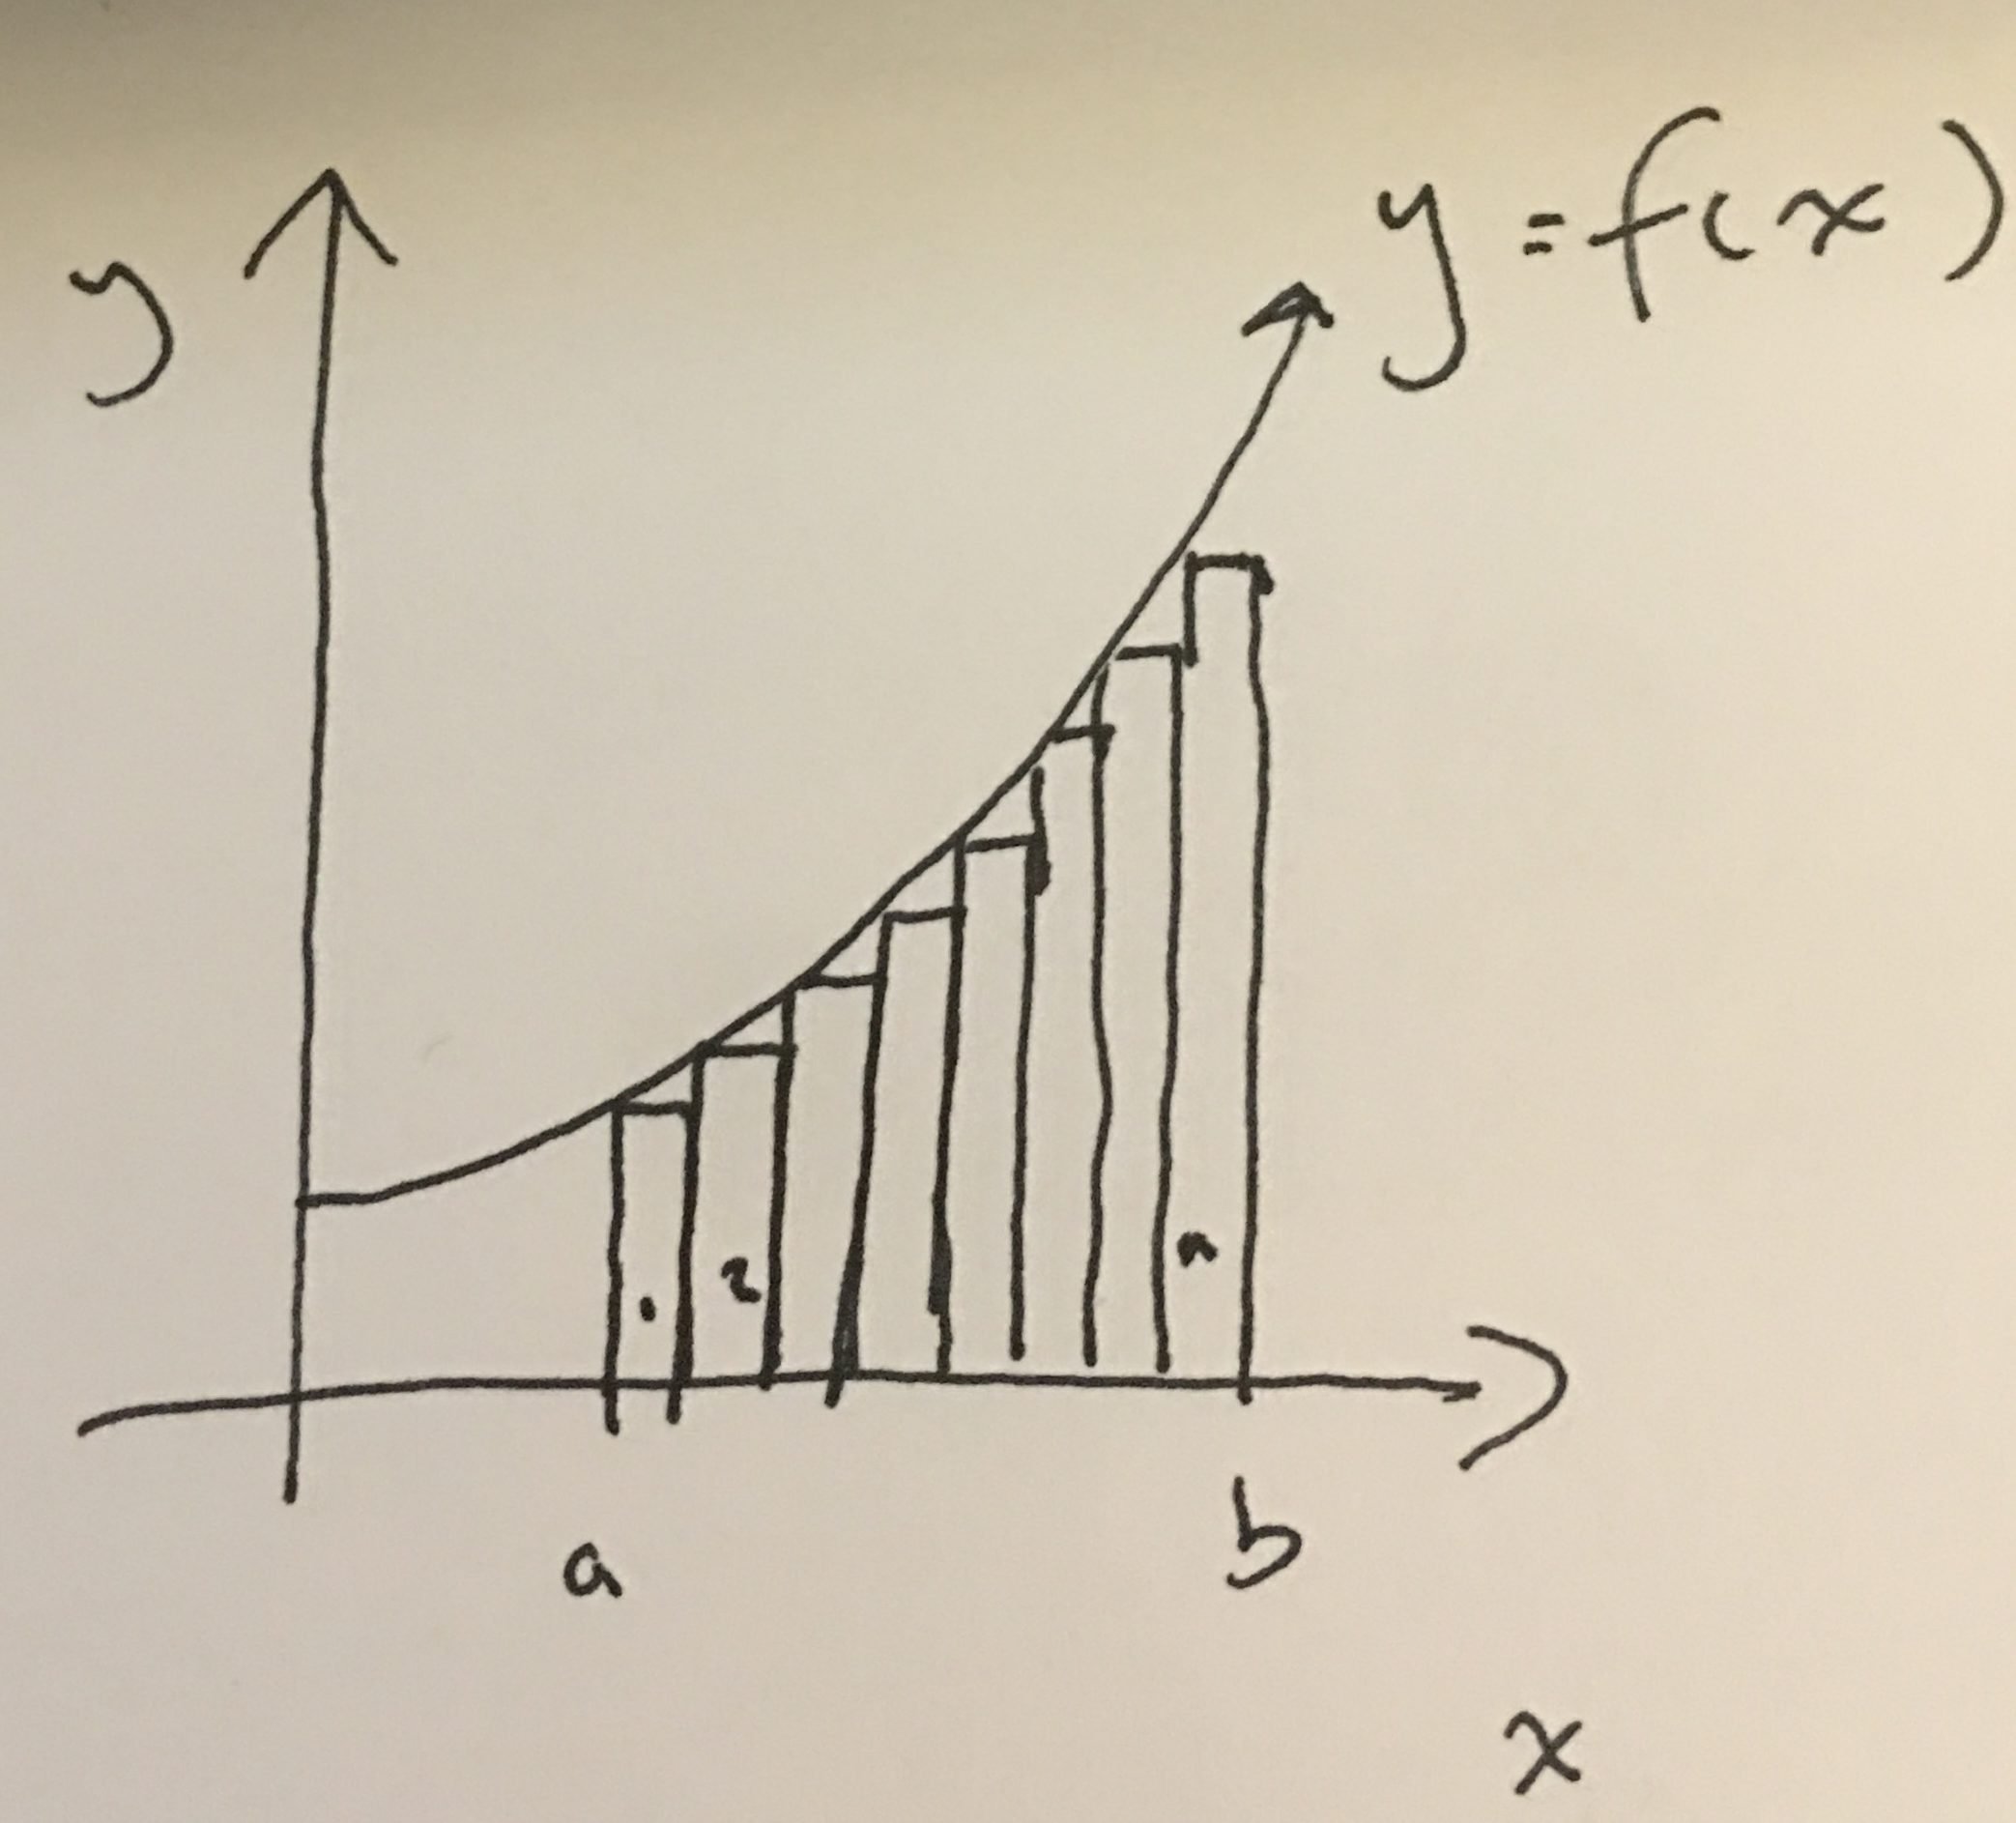
\includegraphics[scale = 0.075]{figures/riemann_ex.png}    
\end{center}

\noindent where $\sum_{u=1}^n f(x_i)\Delta x$ and $\Delta x = \frac{b - a}{n}$. This equals the sum of the area of all the rectangles under $f(x)$. The closer $n$ gets to $\infty$, then the closer the sum of all the areas gets to the area under $f(x)$ from $a$ to $b$. 

\vspace{1em}

\noindent It also turns out that 

\begin{equation*}
    \lim_{n \rightarrow \infty} \sum_{i = 1}^n f(x_i) \Delta x = \int_{b}^a f(x)dx
\end{equation*}

\noindent Because of this, we can use a definite integral to calculate the area under a function/curve between two points.